\documentclass[PICOReport.tex]{subfiles}

\begin{document}

{\bf Inflation and Gravitational waves} \\ %[0.3cm] 
Measurements of the \ac{CMB} together with Einstein's theory of general relativity imply that the observed density perturbations must have been created long before the \ac{CMB} was released, and rather remarkably even before the Universe became filled with a hot and dense plasma of fundamental particles. Understanding the mechanism generating these perturbations, which evolved to fill the Universe with structures, is one of the most important open questions in cosmology.

%While the dynamics of the plasma produces some amount of gravitational waves, the amplitude 
%is predicted to be too small to be detected in existing or planned experiments. 
PICO's precision measurements of temperature and $E$-mode polarization anisotropy will provide additional detailed information about the statistical properties of the primordial density perturbations generated during this epoch. 

The mechanism responsible for the generation of density fluctuations may also produce gravitational waves. PICO will be exquisitely sensitive to the faint imprint that gravitational waves present during recombination leave on the polarization of the CMB. Unlike density perturbations, they not only generate primordial temperature and $E$-mode polarization, but also primordial $B$-mode polarization~\cite{Seljak:1996gy,Kamionkowski:1996zd}. Any detection of primordial $B$-mode polarization by PICO would constitute evidence for gravitational waves from the same primordial period that created the density perturbations and open a new window onto this early epoch.

Because the dynamics of gravitational waves is essentially unaffected by the plasma, they would be a pristine relic from the earliest moments of our Universe, and their properties would shed light on the mechanism that created the primordial perturbations. 
% that grew into the anisotropies of the CMB and the stars and galaxies around us. 
%Knowledge of the strength of the signal and its statistical properties would transform our understanding of many areas of fundamental physics. 


Inflation, a period of nearly exponential expansion of the early Universe~\cite{Guth:1980zm,Linde:1981mu,Albrecht:1982wi,Starobinsky:1980te}, is the leading paradigm explaining the origin of the primordial density perturbations~\cite{Mukhanov:1981xt,Guth:1982ec,Hawking:1982cz,Starobinsky:1982ee,Bardeen:1983qw}. It predicts a nearly scale-invariant spectrum of primordial gravitational waves originating from quantum fluctuations~\cite{Starobinsky:1979ty}. In this sense, a detection of primordial $B$-modes would be the first observation of a phenomenon associated with quantum gravity~\cite{Krauss:2013pha}.

Because the spectrum is scale-invariant, one may hope to detect primordial gravitational waves over a wide range of frequencies including, for example, at LIGO or LISA frequencies. However, as a consequence of the expansion of the Universe, the energy density in the gravitational waves rapidly dilutes with increasing frequency, and observations of the CMB provide the easiest, and for the foreseeable future only way to detect gravitational waves at this scale. 

\begin{figure}[!thb]
\centering
\hspace{-0.15in}
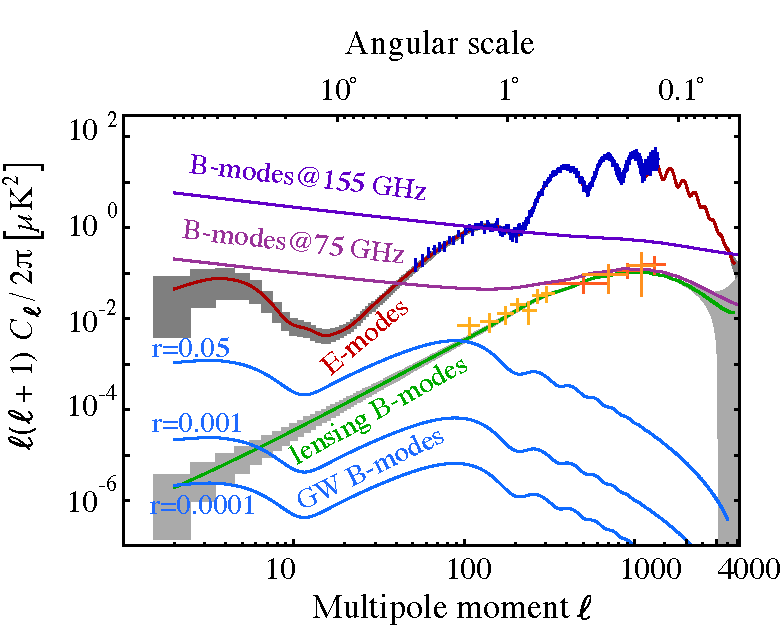
\includegraphics[width=3in]{images/cmb_powspec_PICOv4p1_v2.pdf}
\hspace{-0.15in}
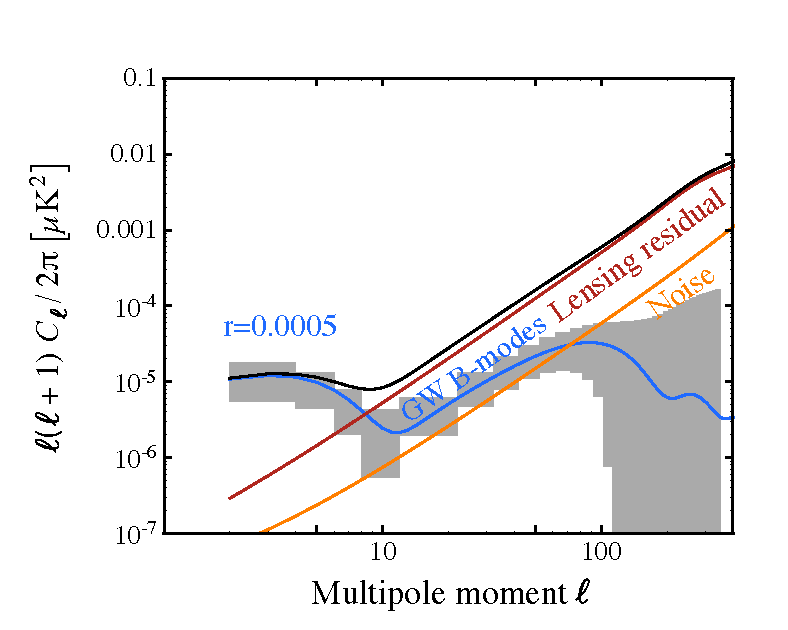
\includegraphics[width=2.9in,trim= 0cm 0.2cm 0cm 0cm]{images/cmbbb_powspec_PICOv4p1.pdf}
\caption{{\em Left panel:} $EE$ (red) and lensing $BB$ (green) angular power spectra and their measurement uncertainties predicted for PICO (gray), as well as the $BB$ power spectrum produced by \ac{IGW} with different values of $r$. Also shown are measurements of lensing from current experiments (orange) and \planck~measurements of the $E$ mode (dark blue)~\citep{PB_BB, keisler2015, actpol_lensing_BB, Array:2015xqh, Planck2018_I}. The $BB$ spectra of Galactic emission on the cleanest $60\%$ of the sky at 75 and 155 GHz (purple) dominate the cosmological signals except at $\ell=1000$ and over a narrow frequency band. 
%At 75 GHz galactic synchrotron emission and polarized emission by thermal dust dominate on large angular scales, lensing dominates around $\ell=1000$. At 155 GHz polarized emission by thermal dust dominates on all scales. 
{\em Right panel:} Predicted uncertainties for a detection of primordial gravitational waves with $r=0.0005$ for PICO (gray), together with the signal (blue), the instrumental noise (orange), and the lensing residual after internal delensing (red).}
\label{fig:clbb}
\end{figure}


The strength of the signal, often quantified by the tensor-to-scalar ratio $r$, is a direct measure of the expansion rate of the Universe during inflation. Together with the Friedmann equation, this reveals one of the most important characteristics of inflation, its energy scale. PICO's goal is to detect primordial gravitational waves if inflation occurred at an energy scale of at least $4\times 10^{15}\,\rm{GeV}$, or equivalently a tensor-to-scalar ratio of $r=3\times 10^{-4}$. 
A detection would have profound implications for fundamental physics because it would provide evidence for a new energy scale tantalizingly close to the energy scale associated with grand unified theories, and would allow us to probe physics at energies far beyond the reach of terrestrial colliders.

Even in the absence of a detection PICO's measurements would contain invaluable information about the early Universe. There are only two classes of slow-roll inflation in agreement with current data that naturally explain the observed value of the spectral index of primordial fluctuations $n_s$. The first class is characterized by potentials of the form $V(\phi)\propto\phi^p$. This class includes many of the simplest models of inflation, some of which have already been strongly disfavored by existing observations (Fig.~\ref{fig:clbb}, right panel). If the constraints on the spectral index tighten by about a factor two with the central value unchanged, and the upper limits on $r$ improve by an order of magnitude, this class would be ruled out. Select models in this class are shown as blue lines in Fig.~\ref{fig:nsr}

The second class is characterized by potentials that approach a constant as a function of field value, either like a power law or exponentially. Two representative examples in this class are shown as the green and gray bands in Fig.~\ref{fig:nsr}. This class also includes $R^2$ inflation, which predicts a tensor-to-scalar ratio of $r\sim 0.004$. All models in this class with a characteristic scale in the potential that is larger than the Planck scale predict a tensor-to-scalar ratio of $r\gtrsim 0.001$. Different values of characteristic scales are indicated by the darker lines in Fig.~\ref{fig:nsr}. Many microphysical models in this class possess a characteristic scale that is super-Planckian, but there are models such as the Goncharov-Linde model with a somewhat smaller characteristic scale that predict a tensor-to-scalar ratio of $r\sim 4\times 10^{-4}$~\cite{Goncharov:1983mw}. 
\begin{figure}[!thb]
\parbox{4.5in}{\centerline{
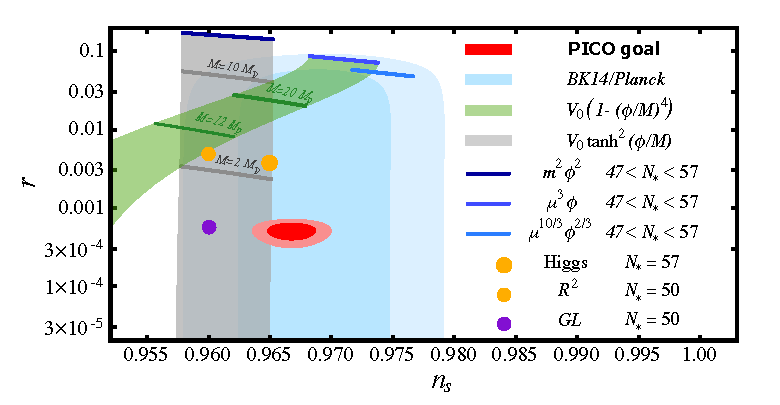
\includegraphics[width=4.5in]{images/nsrlabeledrp0005_PICOv4p1.pdf}}}
\parbox{1.8in}{
\caption{Current 1 and 2$\sigma$ limits on $r$ and $n_{\rm s}$ (blue) and forecasted constraints for a fiducial model with $r = 0.0005$ for PICO. Also shown are predictions for the selected models of inflation discussed in the text.
}
\label{fig:nsr}}
\end{figure}

In the absence of a detection, PICO will limit the amount of gravitational waves to $r<10^{-4}$ at $95\%$ CL and will exclude all these models. 

Let us now take a closer look at the signal. As shown in Fig.~\ref{fig:clbb}, it has two contributions, one on degree angular scales or multipoles of $\ell~\sim~80$, typically referred to as the recombination peak, and another contribution for multipoles of $\ell\lesssim 10$ from the epoch of reionization. 

The contribution from reionization is expected to be brightest relative to the `lensing' $B$-modes created from $E$-modes by the deflection of photons by large-scale structure on their way to us from the surface of last scattering. However, no sub-orbital experiment has yet measured modes at $\ell<40$. The temporal stability, absence of atmospheric noise, and full-sky coverage offered by a satellite like PICO make it the most suitable instrument to reach these lowest multipoles and detect the reionization `bump.'


When the tensor-to-scalar ratio $r \simeq 0.01$, the $BB$ lensing power spectrum and the primordial $BB$ power spectrum are comparable around the recombination peak. For lower levels of $r$, the lensing $B$-modes dominate, but the $B$-mode maps can be "delensed"~\citep{2004PhRvD..69d3005S,2012JCAP...06..014S}. The effect of lensing on $E$ and $B$ maps can be determined and undone if these maps are measured with few-arcmin resolution and sufficient depth. Forecasts for PICO show that at least 73\% of the lensing $B$-mode power can be removed for the baseline configuration, after accounting for foreground subtraction. As much as 80\% will be removed if the foregrounds do not degrade the inherent \ac{SNR} significantly, rising to 85\% for the CBE configuration. Delensing will improve PICO's determination of $r$ by a factor of five to six. We emphasize that PICO will be relying on its own data to conduct the delensing and foreground cleaning, thus avoiding reduced efficacy arising from the need to cross-calibrate experiments, identify common observing areas on the sky, not having frequency-band coverage at the appropriate resolution to remove foregrounds, or from other systematic uncertainties.

Models of the early Universe  differ in their predictions for the scalar spectral index $n_{\rm s}$ and its scale dependence, often referred to as the running of the spectral index $n_{\rm run}$. With its high resolution and low noise levels, PICO will improve the constraints on $n_{\rm s}$ and $n_{\rm run}$ by a factor of about two. In addition, PICO will probe the statistical properties of the primordial fluctuations over a wide range of scales with exquisite precision and improve constraints on departures from Gaussianity by a factor of two to three. By cross-correlating the lensing map with large-scale structure data from LSST it may even be possible to reach a theoretically important threshold (see, e.g.~\cite{2014arXiv1412.4671A} and references therein) and constrain local non-Gaussianity to better than $\sigma(f_{NL})=1$. This is discussed in more detail in section~\ref{gravitationallensing}.


\vspace{0.1in}
%%%%%%%%%%%%%%%%%%%%%%%%%
\parindent = 0pt
{\bf Fundamental Particles: Light relics, Dark Matter, and Neutrinos} \\ %[0.3cm]
\parindent = 15pt
%\vspace{0.1in}
%%%%%%%%%%%%%%%%%%%%%%%%%
$\bullet$ {\bf Light Relics} \hspace{0.1in} In the inflationary paradigm, the Universe was reheated to temperatures of 
at least 10 MeV and perhaps as 
high as $10^{12}$ GeV.  At these high temperatures, even very weakly interacting or very massive particles, 
such as those arising in extensions of the Standard Model of particle physics, can be produced in large 
abundances~\cite{1979ARNPS..29..313S,Bolz:2000fu}.  As the Universe expands and cools, 
the particles fall out of equilibrium, leaving observable signatures in the CMB power spectra. 
Through these effects the CMB is a sensitive probe of neutrino and of other particles' properties.  

% sensitive probe of the fundamental particle content in the Universe
% large abundance, but not large enough to leave present day signatures? or they decay?
% don't like the words 'extensions of ...' suggests very unlikely things. 

One particularly compelling target is the effective number of light relic particle species $\Neff$. The canonical value with three neutrino families is $\Neff = 3.046$. Additional light particles contribute a universal change to $\Neff$ that is a function only of the decoupling temperature and the effective degrees of freedom of the particle, $g$. Furthermore, the range of $\Delta\Neff$ is quite restricted, even for widely varying decoupling temperatures $T_{F}$ with the range $ 0.027\,g \leq \ \Delta \Neff \leq 0.07\,g$ corresponding to decoupling at higher temperatures during post-inflation reheating (0.027$g$) to lower temperatures shortly prior to the QCD phase transition ($0.07g$).

Performance forecasts for $\Neff$ are shown in Fig.~\ref{fig:Neff_future}.  For an experiment like PICO, which has sufficient resolution to reach cosmic-variance-limited measurement of $EE$ up to $\ell =2300$, the two additional most important parameters for improving constraints are the fraction of sky observed $f_{\rm sky}$ and the noise. Achieving both larger $f_{\rm sky}$ and lower noise are strengths of PICO compared to other platforms. The PICO requirement is to constrain $\Delta \Neff < 0.06$ at 95\%.  The corresponding improvement in reach in $T_{F}$ is shown in the right panel of  Fig.~\ref{fig:Neff_future}.  The large improvement over \planck ($\Delta \Neff < 0.28$, 95\%) corresponds to a factor of 400 improvement in the limit on the decoupling temperature for any particle with spin. 

\begin{figure}[t!]
\begin{center}
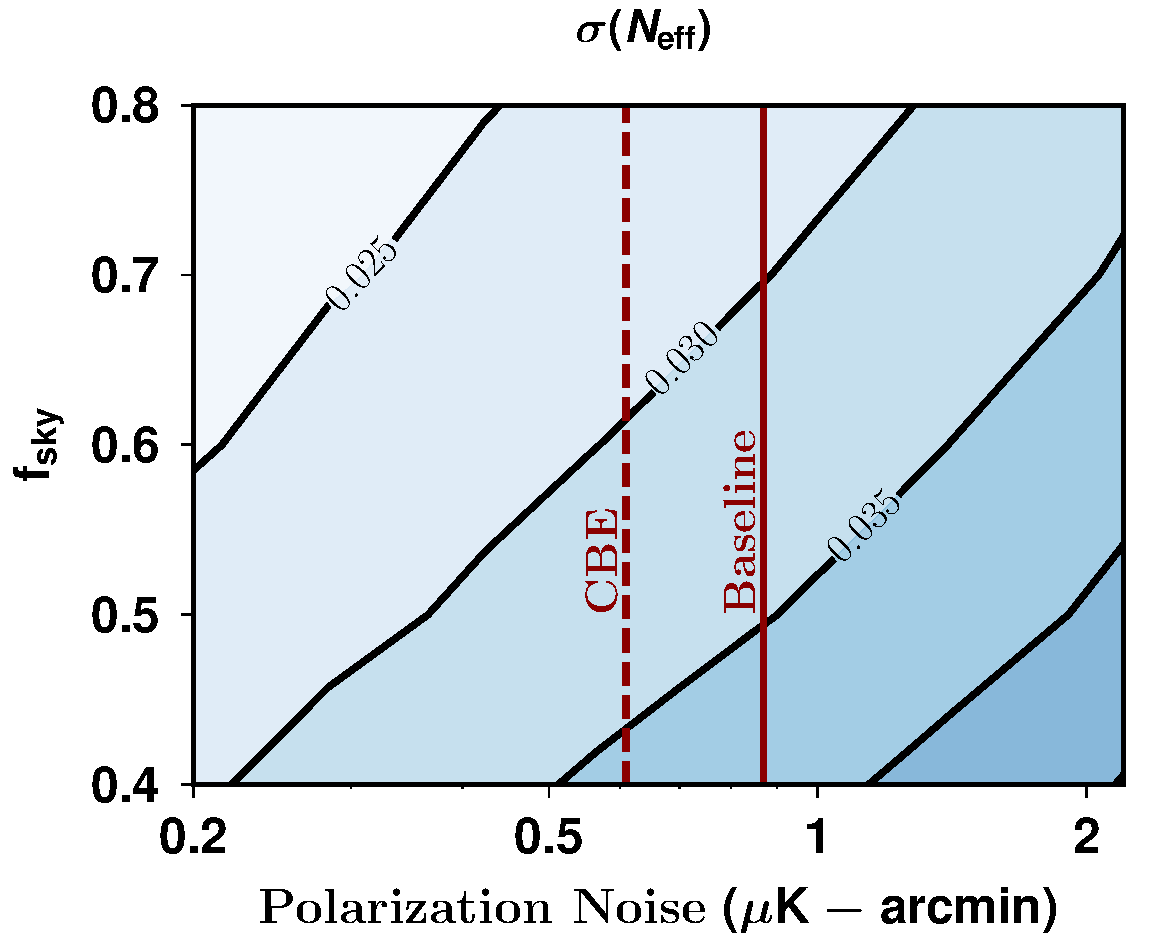
\includegraphics[width=0.45\textwidth]{images/Neff_final.pdf}
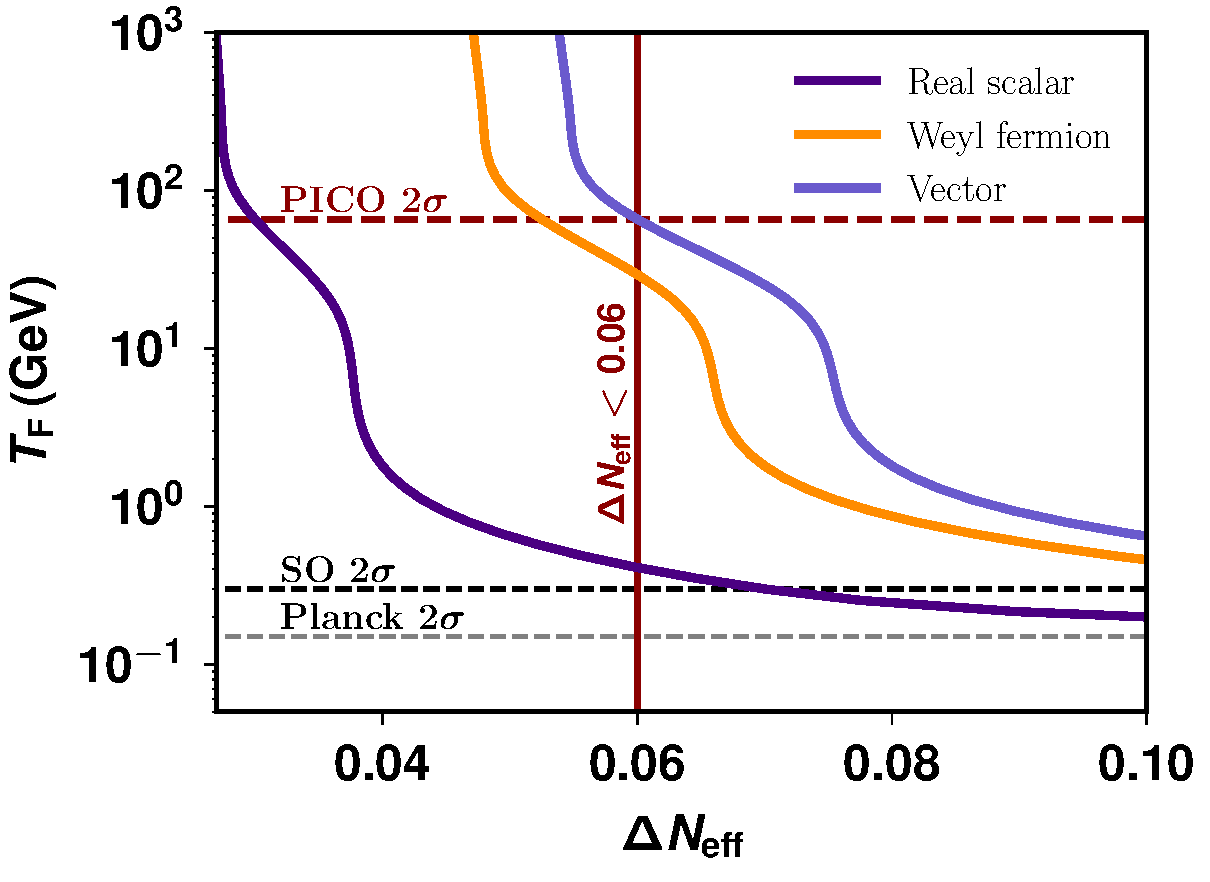
\includegraphics[width=0.47\textwidth]{images/Tf_pico.pdf}
\vspace{-0.15in}
\caption{ \small \setlength{\baselineskip}{0.95\baselineskip}
\textit{Left:} $\Neff$ uncertainty as a function of noise and sky fraction. The resolution assumed is 5'.   Vertical lines denote the expected performance of the baseline mission. \textit{Right:} Reach in the freeze-out temperature for various species, given a measurement of $\Delta \Neff$.  We see that an exclusion of $\Delta \Neff < 0.06$ is a nearly two-order-of-magnitude improvement over \planck and Simons Observatory.  The vertical lines are normalized to the $T_f$ for a single vector particle.
\label{fig:Neff_future}}
\end{center}
\vspace{-0.15in}
\end{figure}

Many light relics of the early Universe are not stable; they decay, leaving faint evidence of their past existence on other tracers. The relics that survive longer than a few minutes, past the epoch of light element synthesis, leave a signature on the helium fraction $Y_p$.  If they decay by the time of recombination, their existence through this period is best measured through the ratio of $\Neff$ to $Y_p$. At both CBE and Baseline sensitivity, PICO can simultaneously measure $\Neff$ and $Y_p$ with $\sigma(\Neff) = 0.08$ and $\sigma(Y_p) =0.005$.  Alternatively, PICO can measure $Y_p$ at fixed $\Neff$ with $\sigma(Y_p) =0.002$ to independently determine the primordial helium abundance with the same precision as astrophysical measurements.  The combination of these measurements is a sensitive test of physics between big bang nucleosynthesis and recombination.  

%%%%%

\noindent$\bullet$ {\bf Dark Matter} \hspace{0.1in} Cosmological measurements have already confirmed the existence of one relic that lies beyond the Standard Model: dark matter. For a conventional WIMP candidate, the CMB places very stringent constraints on its properties through the signature of its annihilation~\cite{Peebles:2000pn, Chen:2003gz, Padmanabhan:2005es}. Most of this information is in the $EE$ power spectrum at $50 < \ell < 300$, which is well-measured by \planck~ and will approach the cosmic-variance limit with existing ground-based surveys~\cite{Madhavacheril:2013cna,Green:2018pmd}.  An entirely complementary way to probe dark matter is to search for evidence of its interactions with other species in cosmological data. Since a lower mass translates to a higher number density of scattering centers, the CMB is particularly useful for probing the low-mass regime and is sensitive to large, nuclear-scale cross sections. 
 
Interactions between dark matter and protons in the early Universe creates a drag force between the two cosmological fluids, damping acoustic oscillations and suppressing power in density perturbations on small scales. As a result, the CMB temperature, polarization, and lensing power spectra are suppressed at high multipoles relative to a Universe without such drag forces.  This effect has been used to search for evidence of dark matter-proton scattering over a range of masses and couplings, and to provide consistency tests of dark matter in the context of the anomalous 21-cm signal reported by the EDGES collaboration~\citep{2002astro.ph..2496C,2004PhRvD..70h3501S,Dvorkin:2013cea,2018PhRvL.121h1301G,2018arXiv180108609B,2018PhRvD..97j3530X,2018arXiv180800001B, 2018PhRvD..98b3013S,2018Natur.555...67B}

%for heavy DM, using CMB and Lyman-$\alpha$ forest measurements~\citep{2002astro.ph..2496C,2004PhRvD..70h3501S,Dvorkin:2013cea}. This analysis has been recently extended to cover wider ranges of masses and couplings~\citep{2018PhRvL.121h1301G,2018arXiv180108609B,2018PhRvD..97j3530X,2018arXiv180800001B, 2018PhRvD..98b3013S}.  These analyses of CMB data have also provided essential consistency tests of dark matter relevant to explaining the anomalous 21-cm signal reported by the EDGES collaboration~\citep{2018Natur.555...67B}.

In Fig. \ref{fig:DM_baryons}, we present current and projected upper limits on the dark matter-proton interaction cross section as a function of dark matter mass, for a spin-independent velocity-independent scattering (chosen as our fiducial model). Regions above the curves are excluded at 95$\%$ confidence. We compare current limits obtained by {\planck} (from \cite{2018PhRvL.121h1301G}) with projections for PICO sensitivity.  We note that PICO can deliver a substantial improvement over the current limits, across the entire dark-matter mass range considered.  Most of the constraining power in the case of PICO (and ground-based next-generation measurements with similar white-noise levels) comes from the measurement of the lensing power spectrum $C_\ell^{\phi \phi}$.
%
\begin{figure}[t]
\begin{center}
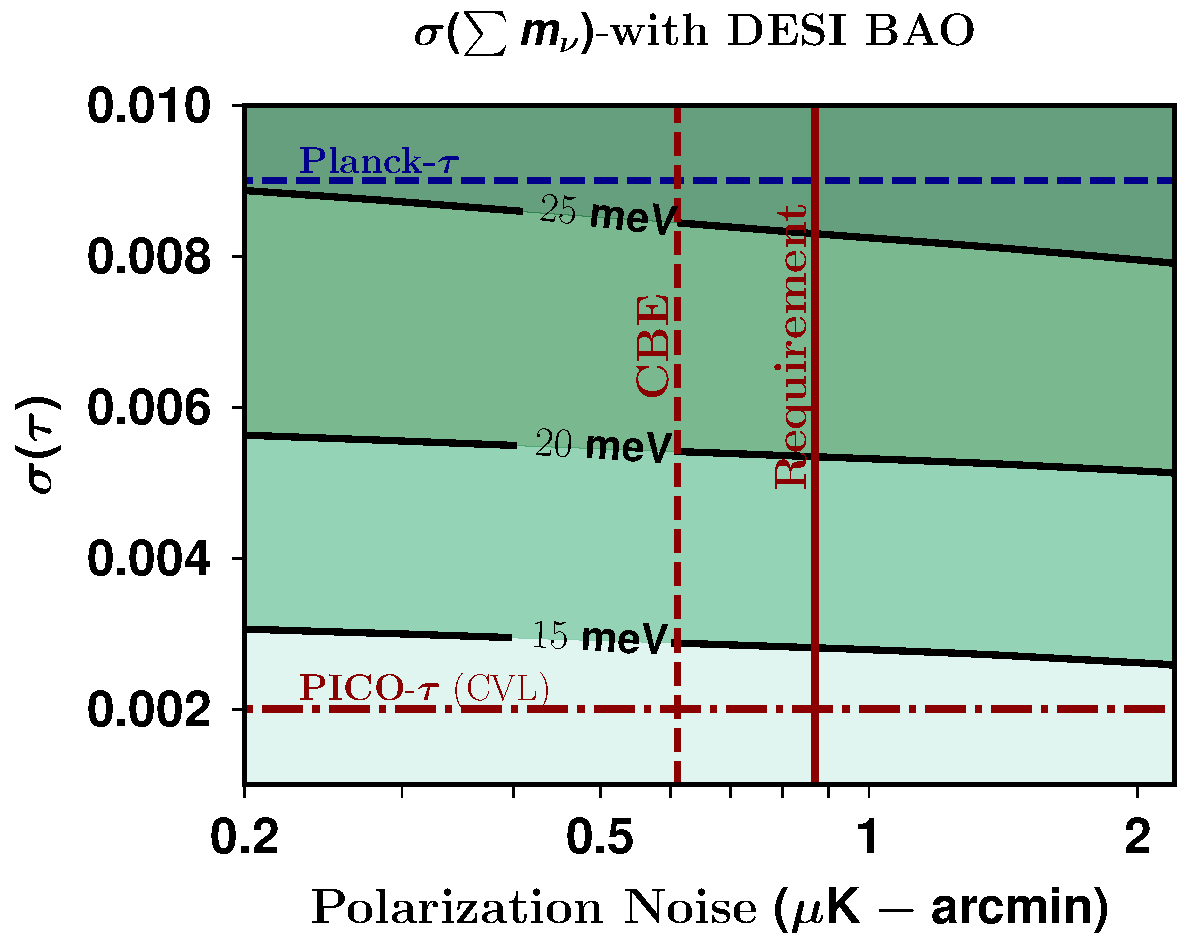
\includegraphics[width=0.48\textwidth]{images/Mnu_tauprior_final.pdf}
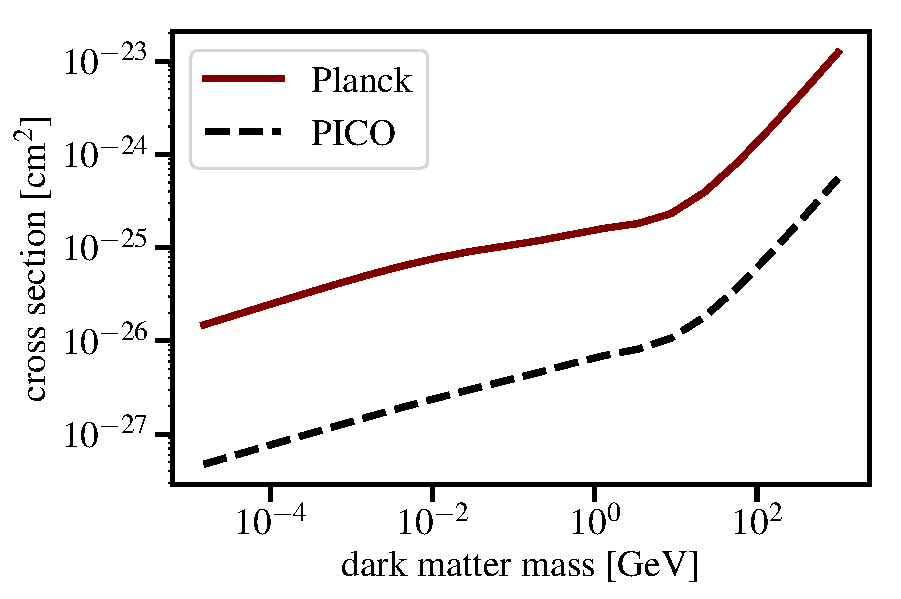
\includegraphics[width=0.50\textwidth]{images/pico_dm_baryon.pdf}
\caption{\textit{Left:}  Forecasts for the uncertainty in the sum of 
neutrino masses, including DESI BAO, as a function of noise and the uncertainty in the measurement of $\tau$, 
for 0.7 sky fraction.  The upper blue dashed line is the current \planck~limit; the lower grey dashed line is the limit from cosmic-variance-limited measurement of $\tau$. \textit{Right:} Upper limits on DM-proton interaction cross section as a function of DM mass, for a spin-independent velocity-independent scattering. Areas above the curves are excluded at 95$\%$ confidence-level.
Shown are the current limits from \planck \cite{2018PhRvL.121h1301G} and a forecast for PICO.}\label{fig:DM_baryons}
\end{center}
\vspace{-0.15in}
\end{figure}
%

\noindent$\bullet$ {\bf Neutrino Mass} \hspace{0.1in} \label{neutrino_fundamental} The origin and structure of the neutrino masses is one of the great outstanding  questions about the nature of the Standard Model particles.  Measurements of neutrinos in the lab have revealed much  about the mass differences and mixing angles.  Cosmology offers a  measurement of the sum of the neutrino masses $\sum m_\nu$ through the gravitational influence of the non-relativistic  cosmic neutrinos.  The measurement of $\Neff = 2.99 \pm 0.17$ \cite{Planck2018_VI} already confirms the existence of these neutrinos at $>10\sigma$ and their mass implies that they will contribute to the matter density at low redshifts.  The best current mass constraint arises from a combination of  \planck and BOSS \ac{BAO} giving $\sum m_\nu < 0.12$ eV (95\%) \cite{Planck2018_VI}.

Cosmological measurements are primarily sensitive to the suppression of power on small scales after the neutrinos become non-relativistic, which can be measured via CMB lensing or weak lensing in a galaxy survey.  However, these measurements are limited by our knowledge of the amplitude of the primordial fluctuation power spectrum, $A_s$.  In practice, CMB observations most directly constrain $A_s e^{-2 \tau}$ and thus do not provide a high-precision measurement of either $A_s$ or $\tau$ separately.  

%ONLY CMB NEEDS TAU? I THOUGHT ALL SURVEYS DO?

Although many surveys hope to detect $\sum m_\nu$, any detection of the minimum value expected from particle physics, $\sum m_\nu = 58$~meV, at more than $2 \sigma$ will require a better measurement of $\tau$.  The best constraints on $\tau$ come from $E$ modes with $\ell < 20$, which require measurements over the largest angular scales. To date, the only proven method for such a measurement is from space. The current limit of $\sigma({\tau}) = 0.007$ is from \planck~\cite{planck2016_xlvi}.  Forecasts for a CMB measurement of $\sum m_\nu$ using the lensing $B$-modes~\cite{Kaplinghat:2003bh} are shown in Fig.~\ref{fig:DM_baryons}.  With the current uncertainty in $\tau$ one is limited to  $\sigma(\sum m_\nu) \gtrsim 25$ meV (after including \ac{BAO}); no other survey or cosmological probe would improve this constraint. However PICO will reach the cosmic-variance limit uncertainty on $\tau$, $\sigma(\tau) \sim 0.002$, and will therefore reach $\sigma(\sum m_\nu) < 15$ meV when combined with measurements of \ac{BAO} from DESI or Euclid~\cite{Levi:2013gra}.  Robustly detecting neutrino mass at  $> 3\sigma$ in any cosmological setting is only possible with an improved measurement of $\tau$, like the one achievable with PICO. This measurement will give $\sum m_\nu>0$ at greater than $4\sigma$ or would exclude the inverted hierarchy ($\sum m_\nu > 100$ meV) at 95\% confidence, depending on the central value of the measurement.  Lab-based measurement could determine the hierarchy before PICO, but only cosmology can measure $\sum m_\nu$.

%%%%%%%%%%%%%%%%%%%%%%%%%
\vspace{0.1in}
\parindent = 0pt
{\bf Fundamental Fields: Primordial Magnetic Fields and Cosmic Birefringence} \\ %[0.3cm]
\parindent = 15pt
%%%%%%%%%%%%%%%%%%%%%%%%%
$\bullet$ {\bf Primordial Magnetic Fields} \hspace{0.1in} One of the long-standing puzzles in astrophysics is the origin of observed 1-10~$\mu$G strength of the magnetic fields of galaxies~\cite{Widrow:2002ud}. Producing such fields through a dynamo mechanism requires a primordial seed field~\cite{Widrow:2011hs}. Moreover, $\mu$G-strength fields have been observed in proto-galaxies that are too young to have gone through the number of revolutions necessary for the dynamo to work. A primordial magnetic field (PMF), present at the time of galaxy formation, could provide the seed or even eliminate the need for the dynamo altogether. Specifically,  a roughly 0.1~nG field in the intergalactic plasma would be adiabatically compressed in the collapse to form a $\sim$1~$\mu$G galactic field \cite{Grasso:2000wj}.
PMFs could have been generated in the aftermath of phase transitions in the early Universe~\cite{Vachaspati:1991nm}, during inflation~\cite{Turner:1987bw,Ratra:1991bn}, or at the end of inflation~\cite{DiazGil:2007dy}. A detection of PMFs with the CMB would be a major discovery as it would establish the field's primordial origin, signal new physics beyond standard models of particle physics and cosmology, and discriminate among different theories of the early Universe~\cite{Barnaby:2012tk,Long:2013tha,Durrer:2013pga}. 

The current CMB bounds on PMF strength are $B_{\rm 1Mpc}<1.2$ nG at 95\% CL for the scale-invariant~PMF spectrum \cite{Zucca:2016iur}, based on measurements of the $TT$, $TE$, $EE$ and $BB$ spectra. 
%In particular, PMF sourced vector modes contribute to the $BB$ power spectrum at high $\ell$ \cite{Lewis:2004ef}. 
The much more accurate measurement of $BB$ by PICO would only marginally improve the PMF bound because CMB spectra scale as $B^4_{1\rm{Mpc}}$. However, Faraday rotation provides a signature that scales linearly with the strength of PMF~\cite{Kosowsky:1996yc}. It converts $E$ modes into $B$ modes, generating mode-coupling $EB$ and $TB$ correlations. So far this signature was out of reach because prior experiments didn't have sufficient sensitivity. Using Faraday rotation, PICO's sensitivity and resolution would allow us to probe PMFs as weak as 0.1~nG ($1\sigma$), a limit that already includes the effects of imperfect lensing subtraction, Galactic foregrounds~\cite{Oppermann:2011td,De:2013dra,Pogosian:2013dya}, and other systematic effects. With this limit PICO will conclusively rule out the purely primordial (i.e, no-dynamo driven) origin of the largest galactic magnetic fields. \\
%
$\bullet$ {\bf Cosmic Birefringence} \hspace{0.1in}
The simplest model for late-time acceleration of the Universe is with a slowly-evolving scalar field, also called quintessence~\cite{Carroll:1998zi}. Such a field generically couples to electromagnetism through a Chern Simons-like term, and causes linear polarization of photons propagating cosmological distances to rotate. This is known as cosmic birefringence~\cite{Carroll:1998zi}. The birefringence converts primordial $E$-modes into $B$-modes. It thus produces parity-violating $TB$ and $EB$ cross-correlations whose magnitude depends on the statistical properties of the rotation field in the sky~\cite{Kamionkowski:2008fp,Gluscevic:2009mm}. There are no theoretical predictions for the level of birefringence, but if observed, it would be evidence for physics beyond the standard model and a potential probe of dark-energy microphysics~\citep{Gluscevic:2009mm,Caldwell:2011,yadav2009}. Using the sensitivity of only the 155~GHz, PICO will improve current constraints on cosmic birefringence (from POLARBEAR~\cite{Ade:2015cao}) by a factor of 300. The constraints will be even stronger when including all frequency bands.

\end{document}

